\documentclass[tikz, border=10pt]{standalone}
\usepackage{tikz}
\usetikzlibrary{arrows.meta, shapes, positioning}
\usepackage{xcolor}
\definecolor{skyblue}{RGB}{135,206,235}
\tikzset{bigskybluenode/.style={circle, fill=skyblue, draw=black, line width=1pt},smallskybluenode/.style={circle, fill=skyblue, draw=black, line width=0.5pt, minimum size=4pt, inner sep=0pt}}
\definecolor{cyan}{RGB}{0,255,255}
\tikzset{bigcyannode/.style={circle, fill=cyan, draw=black, line width=1pt},smallcyannode/.style={circle, fill=cyan, draw=black, line width=0.5pt, minimum size=4pt, inner sep=0pt}}
\definecolor{brightmaroon}{RGB}{195,33,72}
\tikzset{bigbrightmaroonnode/.style={circle, fill=brightmaroon, draw=black, line width=1pt},smallbrightmaroonnode/.style={circle, fill=brightmaroon, draw=black, line width=0.5pt, minimum size=4pt, inner sep=0pt}}
\begin{document}
    % Graph for 3 attributes
    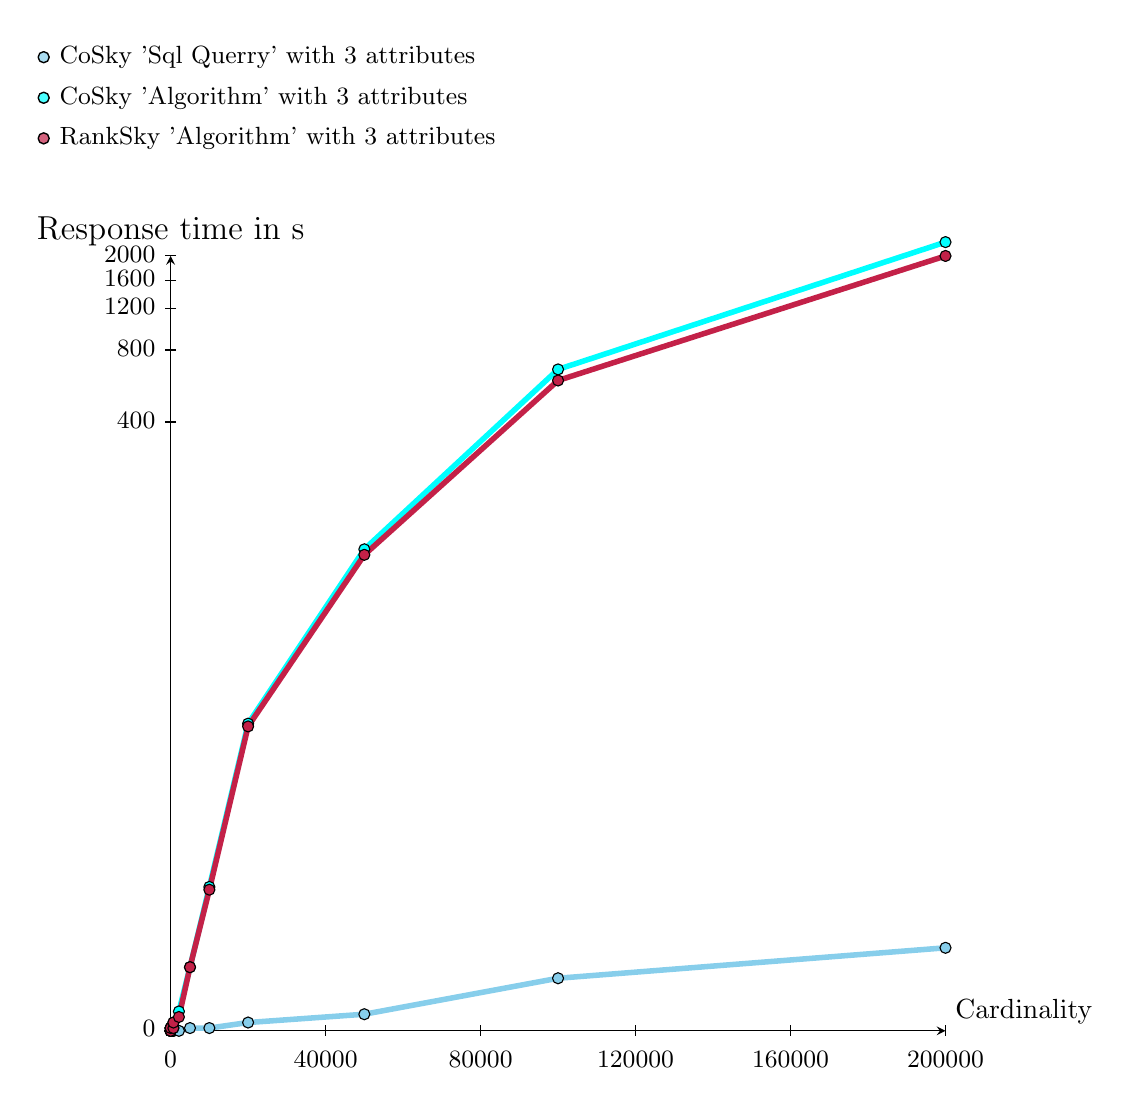
\begin{tikzpicture}[
        line join=bevel,
        smallskybluenode/.style={circle, fill=skyblue, draw=black, line width=0.5pt, minimum size=4pt, inner sep=0pt},
        smallcyannode/.style={circle, fill=cyan, draw=black, line width=0.5pt, minimum size=4pt, inner sep=0pt},
        smallbrightmaroonnode/.style={circle, fill=brightmaroon, draw=black, line width=0.5pt, minimum size=4pt, inner sep=0pt},
    ]
        % Axes
        \draw[-stealth] (0pt, 0pt) -- (280pt, 0pt) node[anchor=north west, yshift=15pt] {Cardinality};
        \draw[-stealth] (0pt, 0pt) -- (0pt, 280pt) node[anchor=south, font=\large] {Response time in s};
        % Axis graduation
        \foreach \x/\xtext in {
            0pt/$0$, 
            56pt/$40000$, 
            112pt/$80000$, 
            168pt/$120000$, 
            224pt/$160000$, 
            280pt/$200000$} {
            \draw (\x, 2pt) -- (\x, -2pt) node[below, font=\small] {\xtext\strut};
        }
        \foreach \y/\ytext in {
            0pt/$0$, 
            220pt/$400$, 
            246pt/$800$, 
            261pt/$1200$, 
            271pt/$1600$, 
            280pt/$2000$} {
            \draw (2pt, \y) -- (-2pt, \y) node[left, font=\small] {\ytext\strut};
        }
        % Lines
        \draw[skyblue, line width=2pt](0pt, 0pt) -- (0pt, 0pt) -- (0pt, 0pt) -- (0pt, 0pt) -- (0pt, 0pt) -- (1pt, 0pt) -- (1pt, 0pt) -- (3pt, 0pt) -- (7pt, 1pt) -- (14pt, 1pt) -- (28pt, 3pt) -- (70pt, 6pt) -- (140pt, 19pt) -- (280pt, 30pt);
        \draw[cyan, line width=2pt](0pt, 1pt) -- (0pt, 0pt) -- (0pt, 1pt) -- (0pt, 1pt) -- (0pt, 1pt) -- (1pt, 1pt) -- (1pt, 3pt) -- (3pt, 7pt) -- (7pt, 23pt) -- (14pt, 52pt) -- (28pt, 111pt) -- (70pt, 174pt) -- (140pt, 239pt) -- (280pt, 285pt);
        \draw[brightmaroon, line width=2pt](0pt, 0pt) -- (0pt, 0pt) -- (0pt, 0pt) -- (0pt, 0pt) -- (0pt, 1pt) -- (1pt, 1pt) -- (1pt, 3pt) -- (3pt, 5pt) -- (7pt, 23pt) -- (14pt, 51pt) -- (28pt, 110pt) -- (70pt, 172pt) -- (140pt, 235pt) -- (280pt, 280pt);
        % Points
        \filldraw[color=black, fill=skyblue] (0pt, 0pt) circle (2pt);
        \filldraw[color=black, fill=skyblue] (0pt, 0pt) circle (2pt);
        \filldraw[color=black, fill=skyblue] (0pt, 0pt) circle (2pt);
        \filldraw[color=black, fill=skyblue] (0pt, 0pt) circle (2pt);
        \filldraw[color=black, fill=skyblue] (0pt, 0pt) circle (2pt);
        \filldraw[color=black, fill=skyblue] (1pt, 0pt) circle (2pt);
        \filldraw[color=black, fill=skyblue] (1pt, 0pt) circle (2pt);
        \filldraw[color=black, fill=skyblue] (3pt, 0pt) circle (2pt);
        \filldraw[color=black, fill=skyblue] (7pt, 1pt) circle (2pt);
        \filldraw[color=black, fill=skyblue] (14pt, 1pt) circle (2pt);
        \filldraw[color=black, fill=skyblue] (28pt, 3pt) circle (2pt);
        \filldraw[color=black, fill=skyblue] (70pt, 6pt) circle (2pt);
        \filldraw[color=black, fill=skyblue] (140pt, 19pt) circle (2pt);
        \filldraw[color=black, fill=skyblue] (280pt, 30pt) circle (2pt);
        \filldraw[color=black, fill=cyan] (0pt, 1pt) circle (2pt);
        \filldraw[color=black, fill=cyan] (0pt, 0pt) circle (2pt);
        \filldraw[color=black, fill=cyan] (0pt, 1pt) circle (2pt);
        \filldraw[color=black, fill=cyan] (0pt, 1pt) circle (2pt);
        \filldraw[color=black, fill=cyan] (0pt, 1pt) circle (2pt);
        \filldraw[color=black, fill=cyan] (1pt, 1pt) circle (2pt);
        \filldraw[color=black, fill=cyan] (1pt, 3pt) circle (2pt);
        \filldraw[color=black, fill=cyan] (3pt, 7pt) circle (2pt);
        \filldraw[color=black, fill=cyan] (7pt, 23pt) circle (2pt);
        \filldraw[color=black, fill=cyan] (14pt, 52pt) circle (2pt);
        \filldraw[color=black, fill=cyan] (28pt, 111pt) circle (2pt);
        \filldraw[color=black, fill=cyan] (70pt, 174pt) circle (2pt);
        \filldraw[color=black, fill=cyan] (140pt, 239pt) circle (2pt);
        \filldraw[color=black, fill=cyan] (280pt, 285pt) circle (2pt);
        \filldraw[color=black, fill=brightmaroon] (0pt, 0pt) circle (2pt);
        \filldraw[color=black, fill=brightmaroon] (0pt, 0pt) circle (2pt);
        \filldraw[color=black, fill=brightmaroon] (0pt, 0pt) circle (2pt);
        \filldraw[color=black, fill=brightmaroon] (0pt, 0pt) circle (2pt);
        \filldraw[color=black, fill=brightmaroon] (0pt, 1pt) circle (2pt);
        \filldraw[color=black, fill=brightmaroon] (1pt, 1pt) circle (2pt);
        \filldraw[color=black, fill=brightmaroon] (1pt, 3pt) circle (2pt);
        \filldraw[color=black, fill=brightmaroon] (3pt, 5pt) circle (2pt);
        \filldraw[color=black, fill=brightmaroon] (7pt, 23pt) circle (2pt);
        \filldraw[color=black, fill=brightmaroon] (14pt, 51pt) circle (2pt);
        \filldraw[color=black, fill=brightmaroon] (28pt, 110pt) circle (2pt);
        \filldraw[color=black, fill=brightmaroon] (70pt, 172pt) circle (2pt);
        \filldraw[color=black, fill=brightmaroon] (140pt, 235pt) circle (2pt);
        \filldraw[color=black, fill=brightmaroon] (280pt, 280pt) circle (2pt);
        % Caption
        \matrix [draw=none, fill=white, fill opacity=0.7, text opacity=1,
                 above right=0.5cm and 0cm of current bounding box.north west,
                 nodes={font=\small, anchor=west}] {
            \node [smallskybluenode, label=right:CoSky 'Sql Querry' with 3 attributes] {}; \\
            \node [smallcyannode, label=right:CoSky 'Algorithm' with 3 attributes] {}; \\
            \node [smallbrightmaroonnode, label=right:RankSky 'Algorithm' with 3 attributes] {}; \\
        };
    \end{tikzpicture}
\clearpage
    % Graph for 6 attributes
    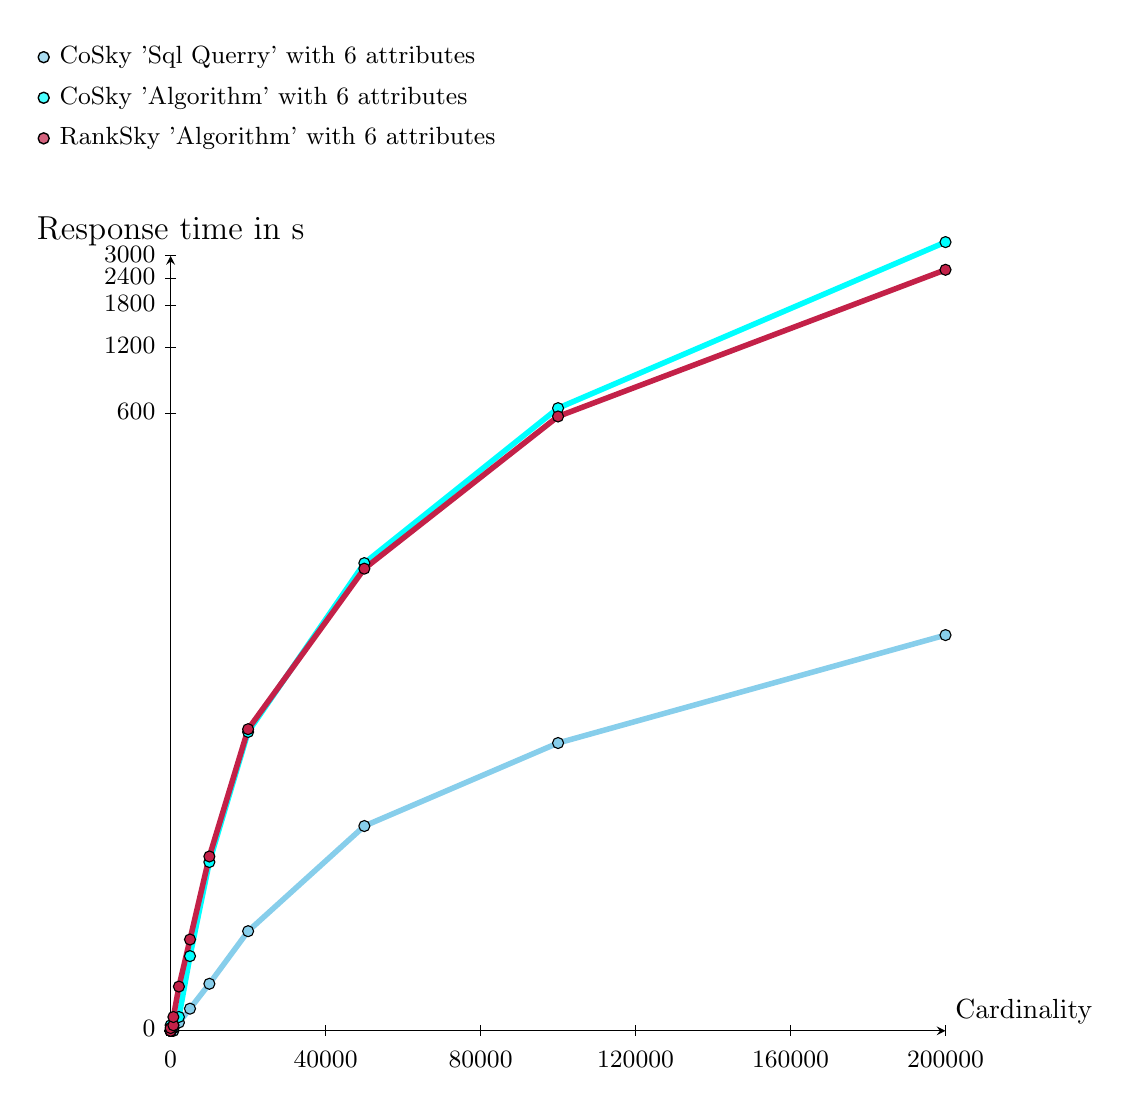
\begin{tikzpicture}[
        line join=bevel,
        smallskybluenode/.style={circle, fill=skyblue, draw=black, line width=0.5pt, minimum size=4pt, inner sep=0pt},
        smallcyannode/.style={circle, fill=cyan, draw=black, line width=0.5pt, minimum size=4pt, inner sep=0pt},
        smallbrightmaroonnode/.style={circle, fill=brightmaroon, draw=black, line width=0.5pt, minimum size=4pt, inner sep=0pt},
    ]
        % Axes
        \draw[-stealth] (0pt, 0pt) -- (280pt, 0pt) node[anchor=north west, yshift=15pt] {Cardinality};
        \draw[-stealth] (0pt, 0pt) -- (0pt, 280pt) node[anchor=south, font=\large] {Response time in s};
        % Axis graduation
        \foreach \x/\xtext in {
            0pt/$0$, 
            56pt/$40000$, 
            112pt/$80000$, 
            168pt/$120000$, 
            224pt/$160000$, 
            280pt/$200000$} {
            \draw (\x, 2pt) -- (\x, -2pt) node[below, font=\small] {\xtext\strut};
        }
        \foreach \y/\ytext in {
            0pt/$0$, 
            223pt/$600$, 
            247pt/$1200$, 
            262pt/$1800$, 
            272pt/$2400$, 
            280pt/$3000$} {
            \draw (2pt, \y) -- (-2pt, \y) node[left, font=\small] {\ytext\strut};
        }
        % Lines
        \draw[skyblue, line width=2pt](0pt, 0pt) -- (0pt, 0pt) -- (0pt, 0pt) -- (0pt, 0pt) -- (0pt, 0pt) -- (1pt, 0pt) -- (1pt, 1pt) -- (3pt, 3pt) -- (7pt, 8pt) -- (14pt, 17pt) -- (28pt, 36pt) -- (70pt, 74pt) -- (140pt, 104pt) -- (280pt, 143pt);
        \draw[cyan, line width=2pt](0pt, 0pt) -- (0pt, 0pt) -- (0pt, 0pt) -- (0pt, 0pt) -- (0pt, 2pt) -- (1pt, 1pt) -- (1pt, 2pt) -- (3pt, 5pt) -- (7pt, 27pt) -- (14pt, 61pt) -- (28pt, 108pt) -- (70pt, 169pt) -- (140pt, 225pt) -- (280pt, 285pt);
        \draw[brightmaroon, line width=2pt](0pt, 0pt) -- (0pt, 0pt) -- (0pt, 0pt) -- (0pt, 0pt) -- (0pt, 1pt) -- (1pt, 2pt) -- (1pt, 5pt) -- (3pt, 16pt) -- (7pt, 33pt) -- (14pt, 63pt) -- (28pt, 109pt) -- (70pt, 167pt) -- (140pt, 222pt) -- (280pt, 275pt);
        % Points
        \filldraw[color=black, fill=skyblue] (0pt, 0pt) circle (2pt);
        \filldraw[color=black, fill=skyblue] (0pt, 0pt) circle (2pt);
        \filldraw[color=black, fill=skyblue] (0pt, 0pt) circle (2pt);
        \filldraw[color=black, fill=skyblue] (0pt, 0pt) circle (2pt);
        \filldraw[color=black, fill=skyblue] (0pt, 0pt) circle (2pt);
        \filldraw[color=black, fill=skyblue] (1pt, 0pt) circle (2pt);
        \filldraw[color=black, fill=skyblue] (1pt, 1pt) circle (2pt);
        \filldraw[color=black, fill=skyblue] (3pt, 3pt) circle (2pt);
        \filldraw[color=black, fill=skyblue] (7pt, 8pt) circle (2pt);
        \filldraw[color=black, fill=skyblue] (14pt, 17pt) circle (2pt);
        \filldraw[color=black, fill=skyblue] (28pt, 36pt) circle (2pt);
        \filldraw[color=black, fill=skyblue] (70pt, 74pt) circle (2pt);
        \filldraw[color=black, fill=skyblue] (140pt, 104pt) circle (2pt);
        \filldraw[color=black, fill=skyblue] (280pt, 143pt) circle (2pt);
        \filldraw[color=black, fill=cyan] (0pt, 0pt) circle (2pt);
        \filldraw[color=black, fill=cyan] (0pt, 0pt) circle (2pt);
        \filldraw[color=black, fill=cyan] (0pt, 0pt) circle (2pt);
        \filldraw[color=black, fill=cyan] (0pt, 0pt) circle (2pt);
        \filldraw[color=black, fill=cyan] (0pt, 2pt) circle (2pt);
        \filldraw[color=black, fill=cyan] (1pt, 1pt) circle (2pt);
        \filldraw[color=black, fill=cyan] (1pt, 2pt) circle (2pt);
        \filldraw[color=black, fill=cyan] (3pt, 5pt) circle (2pt);
        \filldraw[color=black, fill=cyan] (7pt, 27pt) circle (2pt);
        \filldraw[color=black, fill=cyan] (14pt, 61pt) circle (2pt);
        \filldraw[color=black, fill=cyan] (28pt, 108pt) circle (2pt);
        \filldraw[color=black, fill=cyan] (70pt, 169pt) circle (2pt);
        \filldraw[color=black, fill=cyan] (140pt, 225pt) circle (2pt);
        \filldraw[color=black, fill=cyan] (280pt, 285pt) circle (2pt);
        \filldraw[color=black, fill=brightmaroon] (0pt, 0pt) circle (2pt);
        \filldraw[color=black, fill=brightmaroon] (0pt, 0pt) circle (2pt);
        \filldraw[color=black, fill=brightmaroon] (0pt, 0pt) circle (2pt);
        \filldraw[color=black, fill=brightmaroon] (0pt, 0pt) circle (2pt);
        \filldraw[color=black, fill=brightmaroon] (0pt, 1pt) circle (2pt);
        \filldraw[color=black, fill=brightmaroon] (1pt, 2pt) circle (2pt);
        \filldraw[color=black, fill=brightmaroon] (1pt, 5pt) circle (2pt);
        \filldraw[color=black, fill=brightmaroon] (3pt, 16pt) circle (2pt);
        \filldraw[color=black, fill=brightmaroon] (7pt, 33pt) circle (2pt);
        \filldraw[color=black, fill=brightmaroon] (14pt, 63pt) circle (2pt);
        \filldraw[color=black, fill=brightmaroon] (28pt, 109pt) circle (2pt);
        \filldraw[color=black, fill=brightmaroon] (70pt, 167pt) circle (2pt);
        \filldraw[color=black, fill=brightmaroon] (140pt, 222pt) circle (2pt);
        \filldraw[color=black, fill=brightmaroon] (280pt, 275pt) circle (2pt);
        % Caption
        \matrix [draw=none, fill=white, fill opacity=0.7, text opacity=1,
                 above right=0.5cm and 0cm of current bounding box.north west,
                 nodes={font=\small, anchor=west}] {
            \node [smallskybluenode, label=right:CoSky 'Sql Querry' with 6 attributes] {}; \\
            \node [smallcyannode, label=right:CoSky 'Algorithm' with 6 attributes] {}; \\
            \node [smallbrightmaroonnode, label=right:RankSky 'Algorithm' with 6 attributes] {}; \\
        };
    \end{tikzpicture}
\clearpage
    % Graph for 9 attributes
    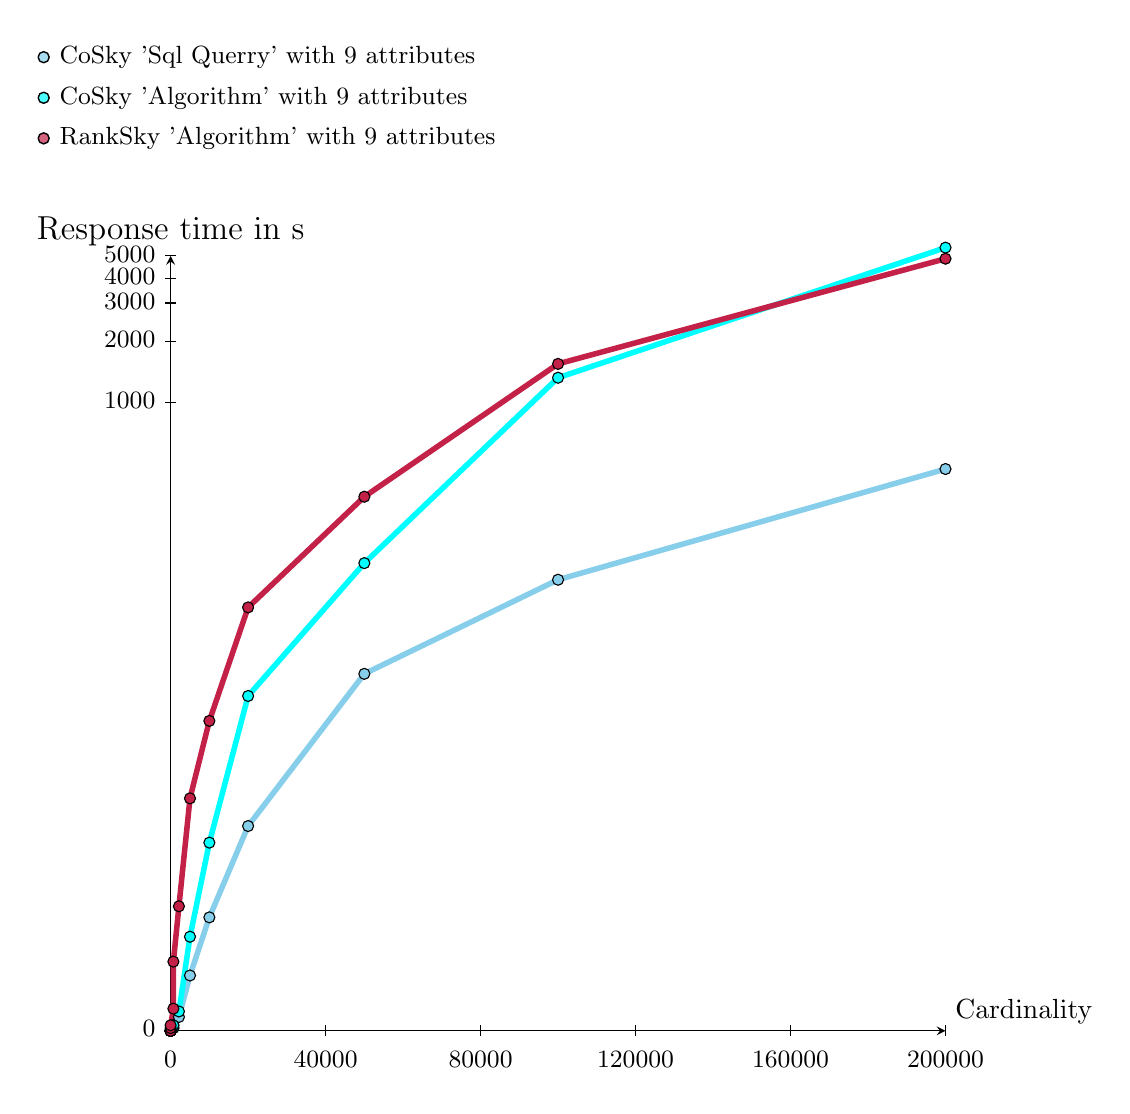
\begin{tikzpicture}[
        line join=bevel,
        smallskybluenode/.style={circle, fill=skyblue, draw=black, line width=0.5pt, minimum size=4pt, inner sep=0pt},
        smallcyannode/.style={circle, fill=cyan, draw=black, line width=0.5pt, minimum size=4pt, inner sep=0pt},
        smallbrightmaroonnode/.style={circle, fill=brightmaroon, draw=black, line width=0.5pt, minimum size=4pt, inner sep=0pt},
    ]
        % Axes
        \draw[-stealth] (0pt, 0pt) -- (280pt, 0pt) node[anchor=north west, yshift=15pt] {Cardinality};
        \draw[-stealth] (0pt, 0pt) -- (0pt, 280pt) node[anchor=south, font=\large] {Response time in s};
        % Axis graduation
        \foreach \x/\xtext in {
            0pt/$0$, 
            56pt/$40000$, 
            112pt/$80000$, 
            168pt/$120000$, 
            224pt/$160000$, 
            280pt/$200000$} {
            \draw (\x, 2pt) -- (\x, -2pt) node[below, font=\small] {\xtext\strut};
        }
        \foreach \y/\ytext in {
            0pt/$0$, 
            227pt/$1000$, 
            249pt/$2000$, 
            263pt/$3000$, 
            272pt/$4000$, 
            280pt/$5000$} {
            \draw (2pt, \y) -- (-2pt, \y) node[left, font=\small] {\ytext\strut};
        }
        % Lines
        \draw[skyblue, line width=2pt](0pt, 0pt) -- (0pt, 0pt) -- (0pt, 0pt) -- (0pt, 0pt) -- (0pt, 0pt) -- (1pt, 1pt) -- (1pt, 2pt) -- (3pt, 5pt) -- (7pt, 20pt) -- (14pt, 41pt) -- (28pt, 74pt) -- (70pt, 129pt) -- (140pt, 163pt) -- (280pt, 203pt);
        \draw[cyan, line width=2pt](0pt, 0pt) -- (0pt, 0pt) -- (0pt, 0pt) -- (0pt, 0pt) -- (0pt, 0pt) -- (1pt, 1pt) -- (1pt, 2pt) -- (3pt, 7pt) -- (7pt, 34pt) -- (14pt, 68pt) -- (28pt, 121pt) -- (70pt, 169pt) -- (140pt, 236pt) -- (280pt, 283pt);
        \draw[brightmaroon, line width=2pt](0pt, 0pt) -- (0pt, 0pt) -- (0pt, 0pt) -- (0pt, 1pt) -- (0pt, 2pt) -- (1pt, 8pt) -- (1pt, 25pt) -- (3pt, 45pt) -- (7pt, 84pt) -- (14pt, 112pt) -- (28pt, 153pt) -- (70pt, 193pt) -- (140pt, 241pt) -- (280pt, 279pt);
        % Points
        \filldraw[color=black, fill=skyblue] (0pt, 0pt) circle (2pt);
        \filldraw[color=black, fill=skyblue] (0pt, 0pt) circle (2pt);
        \filldraw[color=black, fill=skyblue] (0pt, 0pt) circle (2pt);
        \filldraw[color=black, fill=skyblue] (0pt, 0pt) circle (2pt);
        \filldraw[color=black, fill=skyblue] (0pt, 0pt) circle (2pt);
        \filldraw[color=black, fill=skyblue] (1pt, 1pt) circle (2pt);
        \filldraw[color=black, fill=skyblue] (1pt, 2pt) circle (2pt);
        \filldraw[color=black, fill=skyblue] (3pt, 5pt) circle (2pt);
        \filldraw[color=black, fill=skyblue] (7pt, 20pt) circle (2pt);
        \filldraw[color=black, fill=skyblue] (14pt, 41pt) circle (2pt);
        \filldraw[color=black, fill=skyblue] (28pt, 74pt) circle (2pt);
        \filldraw[color=black, fill=skyblue] (70pt, 129pt) circle (2pt);
        \filldraw[color=black, fill=skyblue] (140pt, 163pt) circle (2pt);
        \filldraw[color=black, fill=skyblue] (280pt, 203pt) circle (2pt);
        \filldraw[color=black, fill=cyan] (0pt, 0pt) circle (2pt);
        \filldraw[color=black, fill=cyan] (0pt, 0pt) circle (2pt);
        \filldraw[color=black, fill=cyan] (0pt, 0pt) circle (2pt);
        \filldraw[color=black, fill=cyan] (0pt, 0pt) circle (2pt);
        \filldraw[color=black, fill=cyan] (0pt, 0pt) circle (2pt);
        \filldraw[color=black, fill=cyan] (1pt, 1pt) circle (2pt);
        \filldraw[color=black, fill=cyan] (1pt, 2pt) circle (2pt);
        \filldraw[color=black, fill=cyan] (3pt, 7pt) circle (2pt);
        \filldraw[color=black, fill=cyan] (7pt, 34pt) circle (2pt);
        \filldraw[color=black, fill=cyan] (14pt, 68pt) circle (2pt);
        \filldraw[color=black, fill=cyan] (28pt, 121pt) circle (2pt);
        \filldraw[color=black, fill=cyan] (70pt, 169pt) circle (2pt);
        \filldraw[color=black, fill=cyan] (140pt, 236pt) circle (2pt);
        \filldraw[color=black, fill=cyan] (280pt, 283pt) circle (2pt);
        \filldraw[color=black, fill=brightmaroon] (0pt, 0pt) circle (2pt);
        \filldraw[color=black, fill=brightmaroon] (0pt, 0pt) circle (2pt);
        \filldraw[color=black, fill=brightmaroon] (0pt, 0pt) circle (2pt);
        \filldraw[color=black, fill=brightmaroon] (0pt, 1pt) circle (2pt);
        \filldraw[color=black, fill=brightmaroon] (0pt, 2pt) circle (2pt);
        \filldraw[color=black, fill=brightmaroon] (1pt, 8pt) circle (2pt);
        \filldraw[color=black, fill=brightmaroon] (1pt, 25pt) circle (2pt);
        \filldraw[color=black, fill=brightmaroon] (3pt, 45pt) circle (2pt);
        \filldraw[color=black, fill=brightmaroon] (7pt, 84pt) circle (2pt);
        \filldraw[color=black, fill=brightmaroon] (14pt, 112pt) circle (2pt);
        \filldraw[color=black, fill=brightmaroon] (28pt, 153pt) circle (2pt);
        \filldraw[color=black, fill=brightmaroon] (70pt, 193pt) circle (2pt);
        \filldraw[color=black, fill=brightmaroon] (140pt, 241pt) circle (2pt);
        \filldraw[color=black, fill=brightmaroon] (280pt, 279pt) circle (2pt);
        % Caption
        \matrix [draw=none, fill=white, fill opacity=0.7, text opacity=1,
                 above right=0.5cm and 0cm of current bounding box.north west,
                 nodes={font=\small, anchor=west}] {
            \node [smallskybluenode, label=right:CoSky 'Sql Querry' with 9 attributes] {}; \\
            \node [smallcyannode, label=right:CoSky 'Algorithm' with 9 attributes] {}; \\
            \node [smallbrightmaroonnode, label=right:RankSky 'Algorithm' with 9 attributes] {}; \\
        };
    \end{tikzpicture}
\clearpage
\end{document}